\chapter{Grundlagen}
\label{cha:grundlagen}
Das folgende Kapitel gibt eine Übersicht über die verschiedenen Funktionsweisen eines \textit{Caches}. Darauf aufbauend wird anschließend herausgestellt, welche Art von Speicherung in diesem Projekt umgesetzt wird. Dabei wird ebenfalls auf die verschiedenen Auffassungen des Begriffes \textit{Cache} eingegangen und deren Unterschiede erläutert.
\section{Definition eines Caches}
\label{sec:cache-definition}
Ein \textit{Cache} wird im Allgemeinen als eine Speicherregion oder Puffer verstanden, die besonders schnell erreichbar ist, da oft verwendete Daten zwischengespeichert werden. Somit erkauft man sich durch einen erhöhten Speicherbedarf einen Performancegewinn.
\subsection{Cache-Arten}
\textit{Caches} werden in verschiedenen Umgebungen eingesetzt. Hierbei kann zwischen folgenden Arten unterschieden werden:
\begin{itemize}
\item Memory Cache
\item Internet Browser Cache
\item Disk Caching
\item Server Caching
\end{itemize}
\subsubsection*{\textit{Memory Cache}}
Der \textit{Memory Cache} wird in Computern verwendet, um den sehr schnellen \gls{SRAM} des Rechners auszunutzen. Diese Art macht es sich zunutze, dass Programme immer dieselben Daten oder Befehle ausführen. Bereits errechnete Ergebnisse werden vom Betriebssystem in diesem \textit{Cache} gespeichert, um zum Beispiel darauf aufbauend schnellere Berechnungen vollziehen zu können. Als Alternative würde der \gls{DRAM} zur Verfügung stehen, welcher jedoch langsamer ist.\footcite[Vgl.][S.48f.]{Cache-GummerSommer}
\subsubsection*{\textit{Internet Browser Cache}}
Der \textit{Internet Browser Cache} wird ähnlich, aber in einem anderen Einsatz verwendet. Dieser speichert beliebte Seiten des Benutzers zwischen, um den Seitenaufruf zu beschleunigen. Dabei werden Dateien und \glspl{Request} zu der besuchten Seite gespeichert. Wenn der Benutzer auf die vorherige Seite zurück navigiert, kann der \gls{Browser} viele Dateien wiederverwenden und muss nicht die gesamte Seite nachladen.\footcite{Cache-Techtarget}
\subsubsection*{\textit{Disk Caching}}
\textit{Disk Caching} wird besonders beim Lesen von Festplatten verwendet. Dabei werden Daten im \textit{Memory Buffer} gespeichert. Dieser liegt heutzutage in einem gesonderten Bereich auf der Festplatte. Dieser Bereich kann sich jedoch auch im \ac{RAM} des Computers befinden.\footcite{Cache-Techtarget-DiskCache}
\subsubsection*{\textit{Server Caching}}
Beim \textit{Server Caching} geht es darum, den \textit{Traffic} in einem Netzwerk zu minimieren, indem die meistbesuchten Seiten auf einem \textit{Caching Server} gespeichert werden. Wenn ein Benutzer aus dem Netzwerk eine dieser Seiten aufruft, wird diese Seite aus dem \textit{Cache} zurückgegeben und der Request muss nicht wieder über das Internet geleitet werden, sondern wird direkt im internen Netzwerk beantwortet.\footcite{Cache-ProxyCache}
\subsection{Funktionsweisen von Caches}
\label{ssec:cache-funktionsweisen}
\textit{Caches} lassen sich in zwei unterschiedliche Funktionsweisen unterteilen. Diese werden nachfolgend genauer vorgestellt.
\subsubsection*{Store and Forward}
\label{sssec:cache-store-forward}
Das \textit{Store and Forward}-Prinzip ist eine spezielle Art des \textit{Cachings}, das Netze überbrücken soll, welche Verzögerungen tolerieren. Demgegenüber gibt es die Techniken \textit{Streaming} und Internettelefonie, die keine Verzögerungen in der Verbindung tolerieren.\\
\textit{Store and Forward} ist mit einer \gls{TCP}-Übertragung vergleichbar. Beide Techniken speichern kleinere Datenteile zwischen, um so das gesamte Datum in Gänze zu erhalten.\\
Der Vorteil besteht darin, dass eine Zwischenstation die übertragenen Daten speichert, auf Integrität prüft und, wenn gewünscht, weiterleitet.\footcite{Cache-StoreForward}\\
Soll ein Datum auf der Festplatte gespeichert werden, wird es dazu jedoch sicherheitshalber im Puffer zwischengespeichert. Wird dieses Datum direkt danach abgerufen, ist aber noch nicht auf der Festplatte gespeichert, dann kann das Datum aus dem Puffer geladen werden und die geringe Geschwindigkeit der Festplatte wird dem Anwender nicht bewusst.\footcite{Cache-StoreForwardSOA}
\subsubsection*{Function Cache}
\label{sssec:cache-function-cache}
Beim \textit{Function Cache} oder auch \textit{Memoization} handelt es sich um einen \textit{Cache}, der die Funktionsaufrufe eines Programmes samt Ergebnissen speichert. Diese werden dann in den meisten Fällen für darauf aufbauende Berechnungen oder Aktionen verwendet und sorgen somit für einen enormen Geschwindigkeitsanstieg.\footcite{Cache-Memoization}
%\subsection{Ersetzungsalgorithmen}
%\label{sssec:cache-ersetzungsalgorithmen}
%FIFO, LRU, LRU, Random
\subsection{Definition eines Caches innerhalb dieser Arbeit}
\label{ssec:cache-unsere-definition}
Innerhalb dieser Arbeit wird der Begriff des \textit{Caches} als eine abgewandelte Technik zur lokalen Zwischenspeicherung von Daten auf einem mobilen Gerät verstanden. \\
Die allgemeine Definition geht bei einem \textit{Cache} von einer Performancesteigerung aus (siehe Kapitel \ref{sec:cache-definition}). In diesem Projekt wird das Speichern von Daten jedoch dazu verwendet, um Daten auch offline zur Verfügung zu stellen und damit eine Autonomie vom Server zu erreichen. Die bestehenden Eigenschaften zur Ersetzung von Daten und den verschiedenen Arten der Datenspeicherung werden beibehalten, jedoch im ersten Meilenstein nur rudimentär umgesetzt. Dabei wird eine Art \textit{Store and Forward} umgesetzt. Dagegen wird bevorzugt auf den Server zugegriffen, da dieser als primärer Persistenzspeicher fungiert. \\
Ein \textit{Function Cache} wird nicht umgesetzt, da dieser in diesem Anwendungsfall nicht optimal wäre. Es werden die Daten benötigt, die untereinander auch Beziehungen besitzen. Dabei reicht es nicht aus, die Funktionsaufrufe mit den entsprechenden Daten zu speichern, da man die gespeicherten Daten in einigen Fällen über mehrere Abfragen erhalten würde und diese dann mehrfach gespeichert werden würden. Dieses Problem würde dann die Effizienz des Zwischenspeicherns umgehen.
\section{Allgemeine Umsetzung des Caches}
\label{sec:cache-umsetzung}
Der \textit{Cache} wird in beiden Applikationen als eine lokale Datenbank umgesetzt und spiegelt die Datentypen des Servers in einem möglichst großen Umfang wider (siehe Kapitel \ref{sec:Datenbank-Entwurf} zum Aufbau der Server-Datenbank). Die genaue Umsetzung und Auswahl der Entitäten und Attribute muss entsprechend der Umsetzung und der technischen Möglichkeiten geschehen. Dabei wird jedoch weiterhin auf eine möglichst große Übereinstimmung zwischen den verschiedenen Applikationen geachtet. Somit sind die Entwicklungen besser zu vergleichen und bieten den Autoren damit ein besseres Maß zur Entscheidung, welche Applikation zu einem Messeprototypen weiterentwickelt wird.
\subsection{Aufbau eines Caches innerhalb des Projekts}
\label{ssec:cache-aufbau}
Der \textit{Cache} als solches ist die Kombination aus der Logik, die in der Applikation zur Datenhaltung mit umgesetzt wird, und einer lokalen Datenbank zur Speicherung der Daten. Die Schicht der \textit{Business}-Logik muss dabei Methoden zur Verfügung stellen, um die Daten lokal zu speichern und diese bei Bedarf wieder auslesen zu können.\\
Des Weiteren muss die Logik zur Synchronisierung von Daten zwischen der lokalen und der Server-Datenbank umgesetzt werden. Diese wird im Folgenden allgemein beschrieben.
\subsection{Funktionsumfang eines Caches innerhalb des Projekts}
\label{ssec:cache-unsere-funktionsweise}
Der \textit{Cache} muss die Daten auf demselben Stand halten, wie sie auf dem Server vorliegen. Deshalb bietet es sich an, Daten, die zum Server geschickt werden, auch redundant lokal zu speichern. Genauso verfährt man mit Daten, welche vom Server abgerufen werden. Somit hat man keine unnötigen Abfragen zum Erhalt der Datenkonsistenz zwischen den beiden Ebenen. Diese Strategie hat somit einen positiven Einfluss auf die Performance der Applikationen und entlastet den Server von übermäßigen \textit{Requests}. \\
In dem nachstehenden Sequenzdiagramm (siehe Abbildung \ref{pic:cacheGet}) ist der Ablauf für die Logik des \textit{Caches} bei einem \textit{Get}-Aufruf an den Server zu sehen. Ein Sequenzdiagramm zum Ablauf eines POST-Requests liegt dem Anhang bei (siehe Abbildung \ref{pic:cachePost}).\\
%CacheGet-Bild
\begin{figure}[!h]
\centering
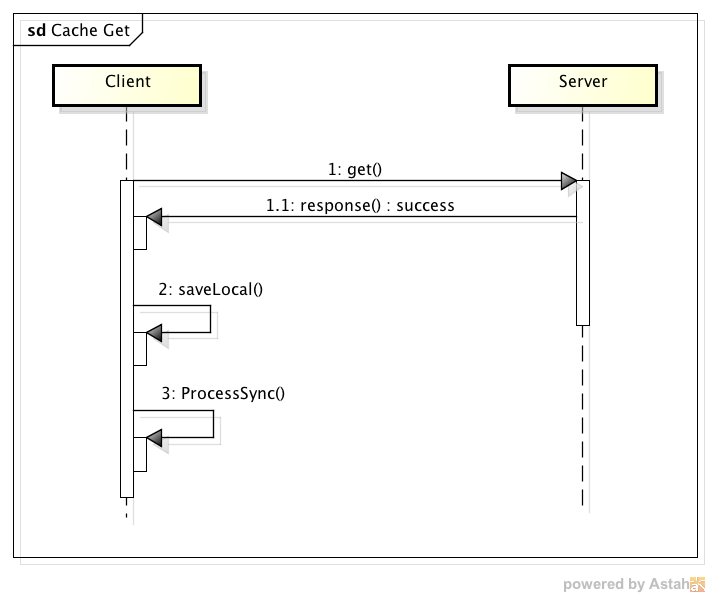
\includegraphics[width=0.8\linewidth]{content/images/Cache-Get}
\caption{Abrufen vom Server}
\label{pic:cacheGet}
\end{figure}
Die Synchronisation soll demnach im Anschluss einer Serververbindung geschehen, da man in diesem Fall sicher sein kann, dass eine Verbindung besteht, die dafür verwendet werden kann. Dementsprechend funktioniert auch der \textit{Post} oder das Hochladen von Daten (siehe Anhang \ref{sec:cachePost}).